\documentclass[a4paper,11pt]{article}
\usepackage{amsmath,amsthm,amsfonts,amssymb,amscd,amstext,vmargin,graphics,graphicx,tabularx,multicol} 
\usepackage[francais]{babel}
\usepackage[utf8]{inputenc}  
\usepackage[T1]{fontenc} 
\usepackage{pstricks-add,tikz,tkz-tab,variations}
\usepackage[autolanguage,np]{numprint} 

\setmarginsrb{1.5cm}{0.5cm}{1cm}{0.5cm}{0cm}{0cm}{0cm}{0cm} %Gauche, haut, droite, haut
\newcounter{numexo}
\newcommand{\exo}[1]{\stepcounter{numexo}\noindent{\bf \underline{Exercice~\thenumexo}}}
\reversemarginpar


\newcounter{enumtabi}
\newcounter{enumtaba}
\newcommand{\q}{\stepcounter{enumtabi} \theenumtabi.  }
\newcommand{\qa}{\stepcounter{enumtaba} (\alph{enumtaba}) }
\newcommand{\initq}{\setcounter{enumtabi}{0}}
\newcommand{\initqa}{\setcounter{enumtaba}{0}}

\newcommand{\be}{\begin{enumerate}}
\newcommand{\ee}{\end{enumerate}}
\newcommand{\bi}{\begin{itemize}}
\newcommand{\ei}{\end{itemize}}
\newcommand{\bp}{\begin{pspicture*}}
\newcommand{\ep}{\end{pspicture*}}
\newcommand{\bt}{\begin{tabular}}
\newcommand{\et}{\end{tabular}}
\renewcommand{\tabularxcolumn}[1]{>{\centering}m{#1}} %(colonne m{} centrée, au lieu de p par défault) 
\newcommand{\tnl}{\tabularnewline}

\newcommand{\bmul}[1]{\begin{multicols}{#1}}
\newcommand{\emul}{\end{multicols}}

\newcommand{\trait}{\noindent \rule{\linewidth}{0.2mm}}
\newcommand{\hs}[1]{\hspace{#1}}
\newcommand{\vs}[1]{\vspace{#1}}

\newcommand{\N}{\mathbb{N}}
\newcommand{\Z}{\mathbb{Z}}
\newcommand{\R}{\mathbb{R}}
\newcommand{\C}{\mathbb{C}}
\newcommand{\Dcal}{\mathcal{D}}
\newcommand{\Ccal}{\mathcal{C}}
\newcommand{\mc}{\mathcal}

\newcommand{\vect}[1]{\overrightarrow{#1}}
\newcommand{\ds}{\displaystyle}
\newcommand{\eq}{\quad \Leftrightarrow \quad}
\newcommand{\vecti}{\vec{\imath}}
\newcommand{\vectj}{\vec{\jmath}}
\newcommand{\Oij}{(O;\vec{\imath}, \vec{\jmath})}
\newcommand{\OIJ}{(O;I,J)}




\newcommand{\reponse}[1][1]{%
\multido{}{#1}{\makebox[\linewidth]{\rule[0pt]{0pt}{20pt}\dotfill}
}}

\newcommand{\titre}[5] 
% #1: titre #2: haut gauche #3: bas gauche #4: haut droite #5: bas droite
{
\noindent #2 \hfill #4 \\
#3 \hfill #5

\vspace{-1.6cm}

\begin{center}\rule{6cm}{0.5mm}\end{center}
\vspace{0.2cm}
\begin{center}{\large{\textbf{#1}}}\end{center}
\begin{center}\rule{6cm}{0.5mm}\end{center}
}



\begin{document}
\pagestyle{empty}
\titre{Chapitre 2 : Les nombres décimaux}{}{}{}{}

\vspace*{1cm}

\begin{center}
{\Large \textbf{Niveau 1 :}}
\end{center}

\vspace*{1cm}

$\rightarrow$ \textbf{Les fractions décimales}\\

\exo \\ Pour chaque figure, écrire la fraction décimale correspondante à la partie coloriée.\\

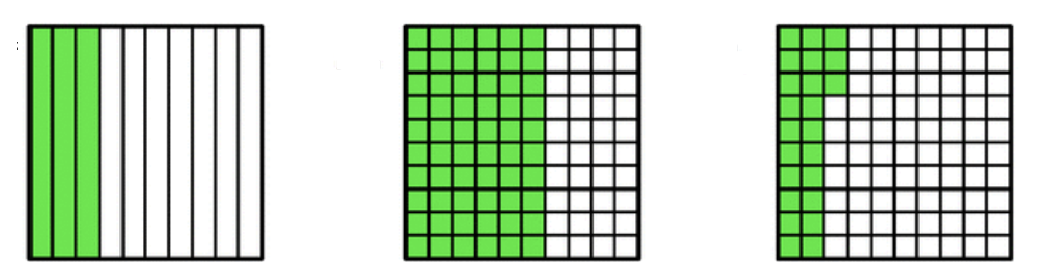
\includegraphics[scale=0.7]{fractiondécimale1.eps} \\

\hspace*{0.7cm} \initqa \qa $\dfrac{. . . . . .}{. . . . . .}$ \hspace*{3cm} \qa $\dfrac{. . . . . .}{. . . . . .}$ \hspace*{2.5cm} \qa $\dfrac{. . . . . .}{. . . . . .}$\\


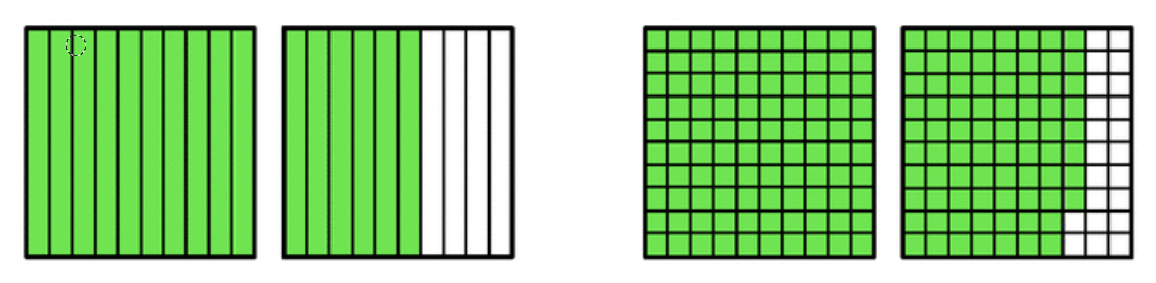
\includegraphics[scale=0.65]{fractiondécimale2.eps} \\

\hspace*{1.5cm} \qa $\dfrac{. . . . . .}{. . . . . .}$ \hspace*{5.5cm} \qa $\dfrac{. . . . . .}{. . . . . .}$\\

\exo \\ Pour chaque figure, écrire la fraction décimale ou la somme d'un entier et d'une fraction décimales correspondant à la partie coloriée.\\

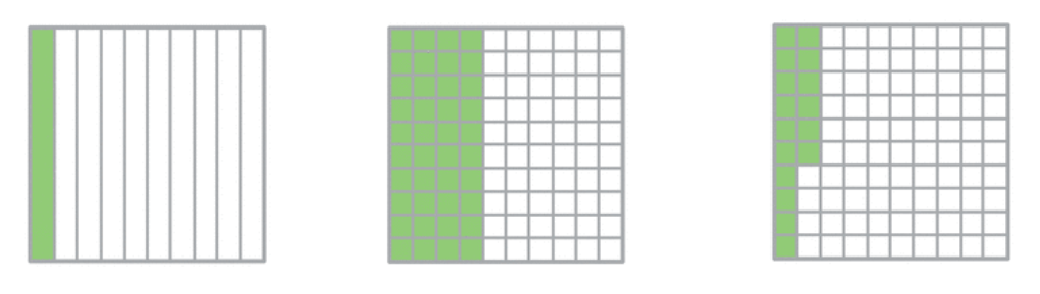
\includegraphics[scale=0.7]{fractiondécimale3.eps} \\

\hspace*{0.8cm} \initqa \qa $\dfrac{. . . . . .}{. . . . . .}$ \hspace*{2.5cm} \qa $\dfrac{. . . . . .}{. . . . . .}$ \hspace*{3cm} \qa $\dfrac{. . . . . .}{. . . . . .}$\\


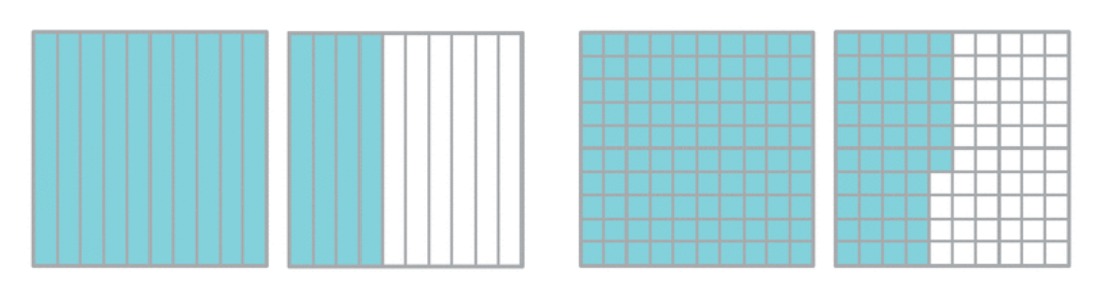
\includegraphics[scale=0.7]{fractiondécimale4.eps} \\

\hspace*{1cm} \qa $\dfrac{. . . . . .}{. . . . . .}= . . . . . . + \dfrac{. . . . . .}{. . . . . .}$ \hspace*{3cm} \qa $\dfrac{. . . . . .}{. . . . . .}= . . . . . . + \dfrac{. . . . . .}{. . . . . .}$\\ 

\exo \\ Écrire sous forme d'une fraction décimale.\\

\initqa \qa $7+\dfrac{2}{10} = ...............$\\

\qa $14 +\dfrac{9}{10} + \dfrac{6}{100}= ...............$\\

\qa $8 +\dfrac{5}{10} + \dfrac{3}{100} + \dfrac{1}{1000}= ...............$\\

\exo \\ Écrire chaque nombre comme la somme d'un entier et d'une fraction décimale inférieure à 1.\\
Exemple : $\dfrac{589}{100} = 5 + \dfrac{89}{100}$\\

\initqa \qa $\dfrac{478}{100} = .................$\\

\qa $\dfrac{82}{10} = .................$\\

\qa $\dfrac{326}{100} = .................$\\

\exo \\ Donner l'écriture décimale de chaque nombre.\\

\initqa \qa Quinze unités et trois dixièmes : ...........................\\

\qa $\dfrac{15}{10}$ = .............\\

\qa Neuf unités et deux centièmes : ...........................\\

\qa $\dfrac{523}{100}$= .............\\

\qa $\dfrac{3}{10}$= .............\\

\exo \\ Écrire la fraction décimale qui correspond à chacun des nombres suivants.\\

\initqa \qa 2,5 = . . . . .\\

\qa 12,9 = . . . . .\\


\qa 5,62 = . . . . .\\

\vspace*{0.5cm}

$\rightarrow$ \textbf{Les zéros inutiles}\\

\exo \\ Écrire les nombres suivants en supprimant si possible les zéros inutiles.\\

\initqa \qa 17,200 = . . . . . . . .\\

\qa 0 021,125 = . . . . . . . .\\

\qa 0,123 0 = . . . . . . . .\\


\qa 01,34 = . . . . . . . .\\

\exo \\ Compléter avec = ou $\neq$ .\\

\initqa 

\qa 1,5 . . . . . . 1,50\\

\qa 10,08 . . . . . . 10,8\\

\qa 04,8 . . . . . . 4,80\\




\vspace*{0.5cm}

$\rightarrow$ \textbf{Position d'un chiffre dans un nombre / partie entière, partie décimale }\\



\exo \\ Dans le nombre 84,7365 :\\

\initqa \qa Le chiffre des dixièmes est : . . . . . . . .\\

\qa Le chiffre des unités est : . . . . . . . .\\

\qa Le chiffre des millièmes est : . . . . . . . .\\

\qa Le chiffre des centaines est : . . . . . . . .\\

\exo \\ On considère le nombre 71,865.\\

\initqa \qa Quelle est la partie entière de ce nombre ?\\

\qa Quelle est la partie décimale de ce nombre?\\

\qa Que représente le chiffre 8? \\

\qa Quel est le chiffre des centièmes ?\\


\vspace*{0.5cm}







\vspace*{0.5cm}

$\rightarrow$ \textbf{Comparaison de deux nombres }\\

\vspace*{0.5cm}

\exo \\ Comparer avec les symboles <, > ou =.\\

\initqa \qa 3,26 . . . . 3,42\\

 \qa 3,35 . . . . 3,3\\
 
  \qa 3,285 . . . . 3,4\\
  
   \qa 3,310 . . . . 3,31\\
   
   
   \exo \\ On considère les nombres suivants : 51,23 ; 51,4 ; 51,184 ; 52\\
   
   \initqa \qa Quel est le plus grand de ces nombres ?\\
   
   \qa Quel est le plus petit de ces nombres?\\
   
   
   \exo \\ Ranger les nombres suivants dans l'ordre croissant (du plus petit au plus grand).\\
      54  \hspace*{1cm} 36,8  \hspace*{1cm}  38,68  \hspace*{1cm} 30,68  \hspace*{1cm} 54,1   \\
   
\hspace*{2cm} . . . .  < . . . . < . . . . < . . . . < . . . .\\

\exo \\ Encadrer chaque nombre par 2 entiers consécutifs.\\

\initqa 

\qa . . . . < 4,5 < . . . .\\

\qa . . . . < 17,06 < . . . .\\

\qa . . . . < 0,98 < . . . .\\


\qa . . . . < 99,1 < . . . .\\

\vspace*{0.5cm}


$\rightarrow$ \textbf{Repérage sur une demi-droite graduée}\\

\exo \\ Pour chaque axe gradué, indiquer les abscisses des points marqués.\\

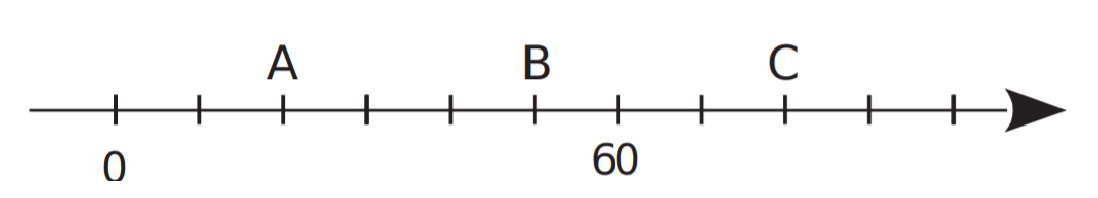
\includegraphics[scale=0.5]{graduee1.eps} \\

A( . . .) \hspace*{1cm} B( . . .)  \hspace*{1cm} C( . . .)\\


\exo \\ Pour chaque axe gradué, indiquer les abscisses des points marqués.\\

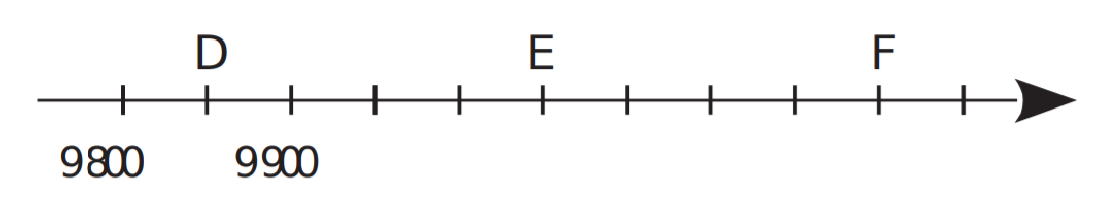
\includegraphics[scale=0.5]{graduee2.eps} \\

D( . . .) \hspace*{1cm} E( . . .)  \hspace*{1cm} F( . . .)\\


\exo \\ Pour chaque axe gradué, indiquer les abscisses des points marqués.\\

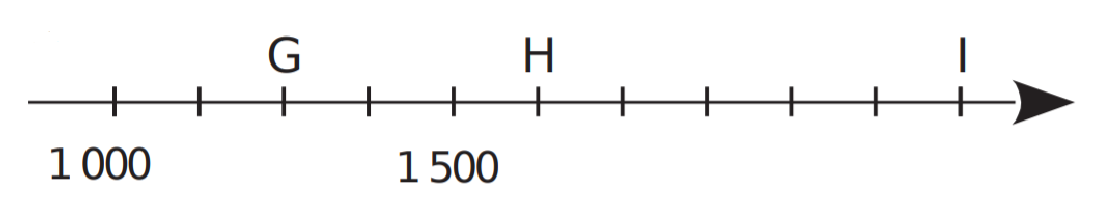
\includegraphics[scale=0.5]{graduee3.eps} \\

G( . . .) \hspace*{1cm} H( . . .)  \hspace*{1cm} I( . . .)\\

\vspace*{0.5cm}

\begin{center}
{\Large \textbf{Niveau 2 :}}
\end{center}

\vspace*{1cm}

$\rightarrow$ \textbf{Les fractions décimales}\\

\exo \\ Décomposer les nombres suivants comme sur l'exemple.\\
Exemple :  $\dfrac{736}{100} = 7 + \dfrac{3}{10} + \dfrac{6}{100}$\\

\initqa 

\qa $\dfrac{81}{10}$\\

\qa  $\dfrac{172}{10}$\\

\qa $\dfrac{953}{100}$ \\

\qa $\dfrac{640}{100}$ \\


\vspace*{0.5cm}

\exo \\ Écrire sous forme d'une fraction décimale.\\

\initqa \qa $ 80 +\dfrac{1}{100}+\dfrac{3}{10} = ............... $\\

\qa $144+\dfrac{6}{10} + \dfrac{8}{1000}= ............... $\\

\qa $9 + \dfrac{7}{1000}= ............... $\\

\exo \\ Écrire chaque nombre comme la somme d'un entier et d'une fraction décimale inférieure à 1.\\
Exemple : $\dfrac{589}{100} = 5 + \dfrac{89}{100}$\\

\initqa 

\qa $\dfrac{152}{10} = .................$\\

\qa $\dfrac{7761}{1000} = .................$\\

\qa $\dfrac{506}{100} = .................$\\

\exo \\ Donner l'écriture décimale de chaque nombre.\\

\initqa \qa Dix unités et deux centièmes : ...........................\\

\qa $3 + \dfrac{2}{10} + \dfrac{3}{100}$ = .............\\

\qa Quatre unités et un millième : ...........................\\

\qa $\dfrac{4789}{1000}$= .............\\

\qa $\dfrac{259}{100}$= .............\\

\exo \\ Écrire la fraction décimale qui correspond à chacun des nombres suivants.\\

\initqa \qa 41,26 = . . . . .\\

\qa 7,125 = . . . . .\\


\qa 9,304 = . . . . .\\


$\rightarrow$ \textbf{Les zéros inutiles}\\

\exo \\ Écrire les nombres suivants en supprimant si possible les zéros inutiles.\\

\initqa \qa 123,201 = . . . . . . . .\\

\qa 0 050,12 = . . . . . . . .\\

\qa 00,609 = . . . . . . . .\\


\qa 654,30 = . . . . . . . .\\

\exo \\ Compléter avec = ou $\neq$ .\\

\initqa 

\qa 0,007 . . . . . . 0,07\\

\qa 93,7 . . . . . . 93,70\\

\qa 24,8 . . . . . . 8,24\\

$\rightarrow$ \textbf{Position d'un chiffre dans un nombre / partie entière, partie décimale }\\

\exo \\ On considère le nombre 1 458,0236.\\

\initqa \qa Quelle est la partie décimale de ce nombre?\\

\qa Que représente le chiffre 3? \\

\qa Quel est le chiffre des dixièmes ?\\

\qa Quel est le chiffre des centièmes ?\\



\exo \\

Je suis un nombre décimal à 5 chiffres.\\
Mon chiffre des centièmes est 8.\\
Mon chiffre des dixièmes  et des centaines est 7.\\
Mon chiffre des unités est 4.\\
Mon chiffres des dizaines est 9.\\
Qui suis-je ?\\



\vspace*{0.5cm}

$\rightarrow$ \textbf{Comparaison de deux nombres }\\

\vspace*{0.5cm}

\exo \\ Comparer avec les symboles <, > ou =.\\

\initqa \qa 8,4 . . . . 6,9\\

 \qa 7,53 . . . . 7,9\\
 
  \qa 11,6 . . . . 11,60\\
  
   \qa 17,3 . . . . 17,27\\
   
   \qa 204 . . . . 20,4\\
   
   
   
   
   
   \exo \\ Ranger les nombres suivants dans l'ordre décroissant (du plus grand au plus petit).\\
     37,7  \hspace*{1cm}37,37  \hspace*{1cm}  3,773  \hspace*{1cm} 7,373 \hspace*{1cm} 3,737  \hspace*{1cm} 7,333   \\
   
\hspace*{2cm} . . . .  > . . . . > . . . . > . . . . > . . . . > . . . .\\

\exo \\ Encadrer chaque nombre par 2 entiers consécutifs.\\

\initqa 

\qa . . . . < 0,758 < . . . .\\

\qa . . . . < 64,30 < . . . .\\

\qa . . . . < 74,586 < . . . .\\


\qa . . . . < 2 399,08 < . . . .\\

\vspace*{0.5cm}

$\rightarrow$ \textbf{Repérage sur une demi-droite graduée}\\

\exo \\ Pour chaque axe gradué, indiquer les abscisses des points marqués.\\

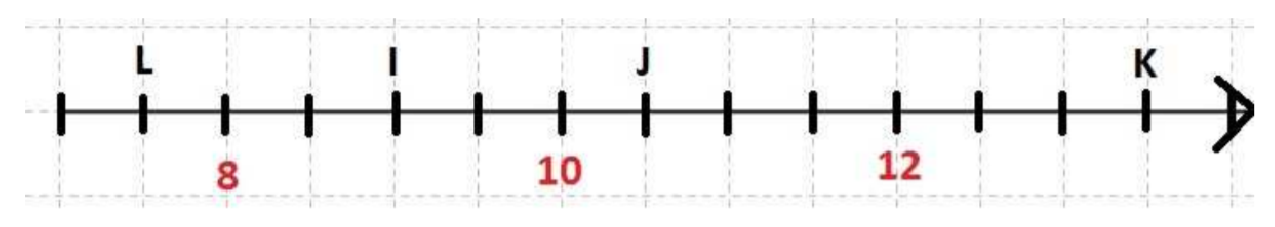
\includegraphics[scale=0.6]{graduee4.eps} \\

L( . . .) \hspace*{1cm} I( . . .)  \hspace*{1cm} J( . . .) \hspace*{1cm} K( . . .)\\


\exo \\ Pour chaque axe gradué, indiquer les abscisses des points marqués.\\

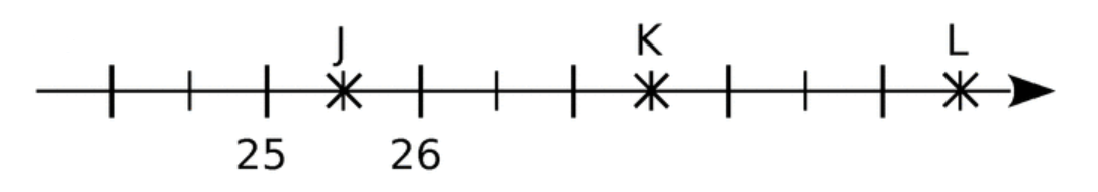
\includegraphics[scale=0.5]{graduee5.eps} \\

J( . . .) \hspace*{1cm} K( . . .)  \hspace*{1cm} L( . . .)\\


\exo \\ Pour chaque axe gradué, indiquer les abscisses des points marqués.\\

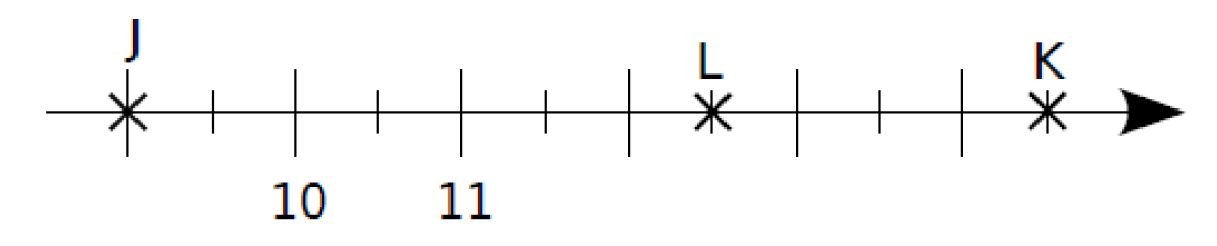
\includegraphics[scale=0.5]{graduee6.eps} \\

J( . . .) \hspace*{1cm} L( . . .)  \hspace*{1cm} K( . . .)\\

\vspace*{0.5cm}

\vspace*{0.5cm}
\begin{center}
{\Large \textbf{Niveau 3 :}}
\end{center}

\vspace*{1cm}

$\rightarrow$ \textbf{Les fractions décimales}\\

\exo \\ Décomposer les nombres suivants comme sur l'exemple.\\
Exemple :  $\dfrac{736}{100} = 7 + \dfrac{3}{10} + \dfrac{6}{100}$\\

\initqa

\qa $\dfrac{178}{100}$\\

\qa  $\dfrac{69}{10}$\\

\qa $\dfrac{4712}{1000}$ \\

\qa $\dfrac{8730}{1000}$ \\

\exo \\ Écrire sous forme d'une fraction décimale.\\

\initqa \qa $ 12+\dfrac{71}{100} = ...............$\\

\qa $5+\dfrac{622}{1000}= ...............$\\

\qa $7 + \dfrac{2}{1000} + \dfrac{4}{10}= ...............$\\

\exo \\ Écrire chaque nombre comme la somme d'un entier et d'une fraction décimale inférieure à 1.\\
Exemple : $\dfrac{589}{100} = 5 + \dfrac{89}{100}$\\

\initqa 

\qa $\dfrac{8947}{100} = .................$\\

\qa $9 + \dfrac{6}{10} + \dfrac{5}{100} = .................$\\

\qa $\dfrac{999}{10} = .................$\\

\exo \\ Donner l'écriture décimale de chaque nombre.\\

\initqa \qa Six cent six unités et douze centièmes : ...........................\\

\qa $75 + \dfrac{2}{10} + \dfrac{9}{100}$ = .............\\

\qa Trois centaines et sept dixièmes : ...........................\\

\qa $\dfrac{158}{1000}$= .............\\

\qa $\dfrac{\text{24 789}}{\text{10 000}}$= .............\\

\exo \\ Écrire la fraction décimale qui correspond à chacun des nombres suivants.\\

\initqa \qa 0,6 = . . . . .\\

\qa 47,06 = . . . . .\\


\qa 4,103 = . . . . .\\

$\rightarrow$ \textbf{Les zéros inutiles}\\

\exo \\ Écrire les nombres suivants en supprimant si possible les zéros inutiles.\\

\initqa \qa 03 005,0 = . . . . . . . .\\

\qa 5,0 = . . . . . . . .\\

\qa 04,001 = . . . . . . . .\\


\qa 30,501 = . . . . . . . .\\

\exo \\ Compléter avec = ou $\neq$ .\\

\initqa 

\qa 2 000 . . . . . . 2,000\\

\qa 05,007 . . . . . . 5,007 0\\

\qa 654,30 . . . . . . 654,300\\


$\rightarrow$ \textbf{Position d'un chiffre dans un nombre / partie entière, partie décimale }\\

\exo \\ Pour chacun des nombres suivants, préciser le rang du chiffre 7.\\

\initqa \qa 575,23 : . . . . . . . . . . . . .\\

\qa 7 025 : . . . . . . . . . . . . .\\

\qa 5,172 : . . . . . . . . . . . . .\\

\qa 0,72 : . . . . . . . . . . . . .\\

\qa 7 : . . . . . . . . . . . . .\\


\exo \\
Je suis un nombre décimal à 4 chiffres.\\
Mon chiffre des dixièmes est 6.\\
Mon chiffre des unités et des centièmes est la moitié de celui des dixièmes.\\
Mon chiffres des millièmes est le tiers de celui des dixièmes.\\
Qui suis-je ?\\

\vspace*{0.5cm}
$\rightarrow$ \textbf{Comparaison de deux nombres }\\

\vspace*{0.5cm}

\exo \\ Comparer avec les symboles <, > ou =.\\

\initqa \qa 05,05 . . . . 5,050\\

 \qa 9,756 . . . . 9,77\\
 
  \qa 0,67 . . . . 0,8\\
  
   \qa 15 . . . . 15,0\\
   
   \qa 52,99 . . . . 52,909\\
   
   
   
   
   
   \exo \\ Ranger les nombres suivants dans l'ordre croissant.\\
     45,12  \hspace*{1cm} 45,21  \hspace*{1cm}  45,201  \hspace*{1cm} 45,012 \hspace*{1cm} 45,102  \hspace*{1cm} 45,2   \\
   
\hspace*{2cm} . . . .  < . . . . < . . . . < . . . . < . . . . < . . . .\\

\exo \\ Encadrer chaque nombre par 2 entiers consécutifs.\\

\initqa 

\qa . . . . < $\dfrac{8523}{100}$ < . . . .\\

\qa . . . . < $\dfrac{15}{10}$ < . . . .\\

\qa . . . . < $\dfrac{36}{10}$ < . . . .\\


\qa . . . . < $\dfrac{342}{100}$ < . . . .\\

$\rightarrow$ \textbf{Repérage sur une demi-droite graduée}\\

\exo \\ Pour chaque axe gradué, indiquer les abscisses des points marqués.\\

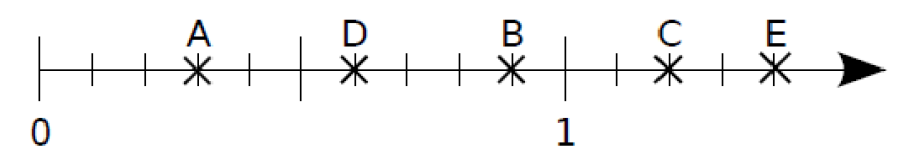
\includegraphics[scale=0.6]{graduee9.eps} \\

A( . . .) \hspace*{1cm} D( . . .)  \hspace*{1cm} B( . . .) \hspace*{1cm} C( . . .)  \hspace*{1cm} E( . . .)\\


\exo \\ Pour chaque axe gradué, indiquer les abscisses des points marqués.\\

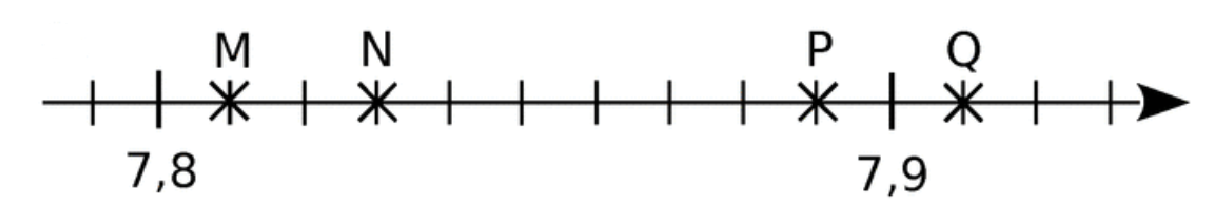
\includegraphics[scale=0.5]{graduee7.eps} \\

M( . . .) \hspace*{1cm} N( . . .)  \hspace*{1cm} P( . . .)  \hspace*{1cm} Q( . . .)\\


\exo \\ Pour chaque axe gradué, indiquer les abscisses des points marqués.\\

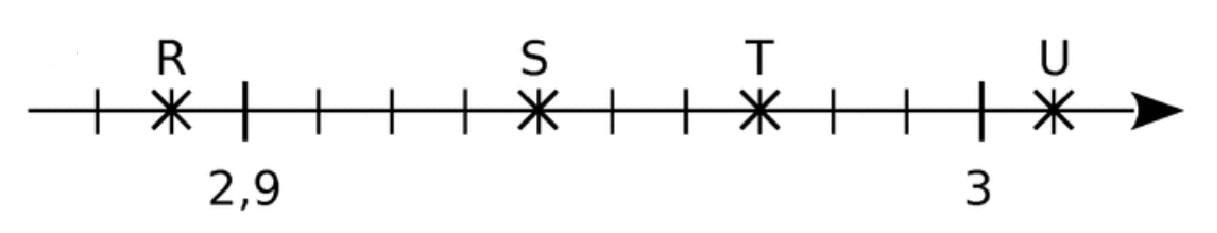
\includegraphics[scale=0.5]{graduee8.eps} \\

R( . . .) \hspace*{1cm} S( . . .)  \hspace*{1cm} T( . . .)  \hspace*{1cm} U( . . .)\\

\vspace*{0.5cm}

\vspace*{0.5cm}
\begin{center}
{\Large \textbf{Niveau 4:}}
\end{center}

\vspace*{1cm}

$\rightarrow$ \textbf{Les fractions décimales}\\

\exo \\ Décomposer les nombres suivants comme sur l'exemple.\\
Exemple :  $\dfrac{736}{100} = 7 + \dfrac{3}{10} + \dfrac{6}{100}$\\

\initqa 

\qa $\dfrac{1253}{100}$\\

\qa  $\dfrac{908}{10}$\\

\qa $\dfrac{543}{1000}$ \\

\qa $\dfrac{32}{1000}$ \\

\exo \\ Écrire sous forme d'une fraction décimale.\\

\initqa \qa $ 14 +\dfrac{7}{10} + \dfrac{26}{1000} = ...............$\\

\qa $\dfrac{4}{10} + \dfrac{5}{100}= ...............$\\

\qa $18 + \dfrac{36}{100}= ...............$\\

\qa $51 + \dfrac{109}{1000}= ...............$\\

\exo \\ Écrire chaque nombre comme la somme d'un entier et d'une fraction décimale inférieure à 1.\\
Exemple : $\dfrac{589}{100} = 5 + \dfrac{89}{100}$\\

\initqa 

\qa $\dfrac{1080}{1000} = .................$\\

\qa $58 + \dfrac{7}{10} + \dfrac{9}{1000} = .................$\\

\qa $4 + \dfrac{236}{100} = .................$\\

\exo \\ Donner l'écriture décimale de chaque nombre.\\

\initqa \qa Cinq centièmes : ...........................\\

\qa $ \dfrac{3}{100} + \dfrac{6}{1000}$ = .............\\

\qa Douze dizaines et onze millièmes : ...........................\\

\qa $\dfrac{15}{100}$= .............\\

\qa $7 +\dfrac{1}{10} + \dfrac{9}{1000}$= .............\\

\exo \\ Écrire la fraction décimale qui correspond à chacun des nombres suivants.\\

\initqa \qa 0,15 = . . . . .\\

\qa 98,005 = . . . . .\\


\qa 250,04 = . . . . .\\

$\rightarrow$ \textbf{Les zéros inutiles}\\

\exo \\ Écrire les nombres suivants en supprimant si possible les zéros inutiles.\\

\initqa \qa 36,700 10 = . . . . . . . .\\

\qa 030,000 = . . . . . . . .\\

\qa 04,602 0 = . . . . . . . .\\


\qa 10 000,010 = . . . . . . . .\\

\exo \\ Compléter avec = ou $\neq$ .\\

\initqa 

\qa 5,000 . . . . . . 5\\

\qa 5 020 . . . . . . 5 020,00\\

\qa 27,06 . . . . . . 27,6\\

$\rightarrow$ \textbf{Position d'un chiffre dans un nombre / partie entière, partie décimale }\\

\exo \\ Dans le nombre 504,872.\\
 
 \initqa 
\qa Quel est le chiffre des dixièmes ? \\

\qa   Quel est le chiffre des millièmes ? \\
 
\qa Quel est le chiffre des dizaines ?   \\

\qa  Quel est le chiffre des centièmes ?  \\

\qa Quel est le nombre de dizaines ?   \\

\qa    Quel est le nombre de millièmes ?   \\

\exo \\ Dans le nombre 32 516, placer la virgule pour que :\\

\initqa  \qa 1 soit le chiffre des unités : . . . . . . . . .\\

\qa 2 soit le chiffre des milliers : . . . . . . . . .\\

\qa 5 soit le chiffre des centièmes : . . . . . . . . .\\

\qa 3 soit le chiffre des dixièmes : . . . . . . . . .\\

\qa 6 soit le chiffre des dizaines : . . . . . . . . .\\
              
\exo \\
Je suis un nombre décimal à 5 chiffres.\\
Mon nombre de dixièmes est 243.\\
Mon chiffre des centièmes est la somme  de celui des unités et celui des dixièmes.\\
Mon chiffre des millièmes est le produit de celui des dizaines par celui des dixièmes.\\
Qui suis-je?\\  

\vspace*{0.5cm}
$\rightarrow$ \textbf{Comparaison de deux nombres }\\

\vspace*{0.5cm}

\exo \\ Comparer avec les symboles <, > ou =.\\

\initqa \qa 7,101 . . . . 7,011\\

 \qa 15,1 . . . . 15,09\\
 
  \qa 0,007 . . . . 0,07\\
  
   \qa 93,7 . . . . 93,700\\
   
   \qa 5,000 . . . . 5\\
   
   
   
   
   
   \exo \\ Ranger les nombres suivants dans l'ordre décroissant.\\
     17,3  \hspace*{1cm} 17,257  \hspace*{1cm}  17,28  \hspace*{1cm} 17,315 \hspace*{1cm} 17,351  \hspace*{1cm} 17,534   \\
   
\hspace*{2cm} . . . .  < . . . . < . . . . < . . . . < . . . . < . . . .\\

\exo \\ Donner un encadrement au dixième près de chaque nombre.\\

\initqa 

\qa . . . . < 64,26 < . . . .\\

\qa . . . . < 1,869 < . . . .\\

\qa . . . . < 458,08 < . . . .\\


\qa . . . . < 489,97 < . . . .\\

$\rightarrow$ \textbf{Repérage sur une demi-droite graduée}\\

\exo \\ Pour chaque axe gradué, indiquer les abscisses des points marqués.\\

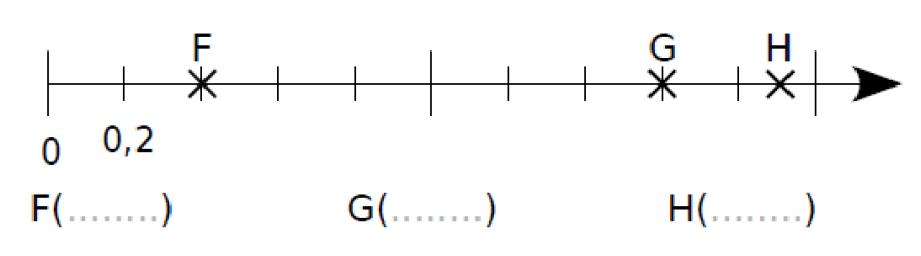
\includegraphics[scale=0.7]{graduee10.eps} \\





\vspace*{0.5cm}

\begin{center}
{\Large \textbf{Niveau 5 :}}
\end{center}

\vspace*{1cm}

$\rightarrow$ \textbf{Les fractions décimales}\\

\exo \\ Compléter avec des chiffres pour que les égalités soient vraies.\\

\initqa \qa $\dfrac{23}{100} + \dfrac{...}{1000}= \dfrac{\text{... ... } 7}{1000}$\\

\qa 5 ...  + $\dfrac{3...}{100} = \dfrac{...83...}{\text{... ... ...}} = \text{... ...} +\dfrac{...}{10} +\dfrac{1}{100}$\\

\qa $\dfrac{1 ...}{10} + \dfrac{...4}{1000}= \dfrac{...41..}{1000}$\\

\exo \\ Écrire sous forme d'une fraction décimale.\\

\initqa \qa $ \dfrac{3}{10} + \dfrac{5}{1000} = ...............$\\

\qa $\dfrac{158}{10} + \dfrac{9}{1000}= ...............$\\

\qa $47  + \dfrac{205}{100}= ...............$\\

\qa $8 + \dfrac{15}{100}= ...............$\\

\exo \\ Écrire chaque nombre comme la somme d'un entier et d'une fraction décimale inférieure à 1.\\
Exemple : $\dfrac{589}{100} = 5 + \dfrac{89}{100}$\\

\initqa 

\qa $\dfrac{5403}{100} = .................$\\

\qa $12 + \dfrac{19}{10} +\dfrac{2}{1000} = .................$\\

\qa $\dfrac{124}{10} + \dfrac{2}{100} +\dfrac{7}{1000} = .................$\\

\exo \\ Donner l'écriture décimale de chaque nombre.\\

\initqa \qa 956 millièmes : ...........................\\

\qa $ \dfrac{4}{10} + \dfrac{8}{1000}$ = .............\\

\qa 9 dixièmes : ...........................\\

\qa $\dfrac{75}{1000}$= .............\\

\qa $ \dfrac{\text{15 384}}{100}$= .............\\

\exo \\ Écrire la fraction décimale qui correspond à chacun des nombres suivants.\\

\initqa \qa 95 = . . . . .\\

\qa 0,0159 = . . . . .\\


\qa 100,08 = . . . . .\\

$\rightarrow$ \textbf{Les zéros inutiles}\\

\exo \\ Écrire les nombres suivants en supprimant si possible les zéros inutiles.\\

\initqa \qa 01 205 500,0 = . . . . . . . .\\

\qa 0,500 = . . . . . . . .\\

\qa 005 401,070 0 = . . . . . . . .\\


\qa 023,201 20 = . . . . . . . .\\

\exo \\ Compléter avec = ou $\neq$ .\\

\initqa 

\qa 03 005 . . . . . . 3 005,0\\

\qa 3 070,02 . . . . . . 307,2\\

\qa 01,807 0 . . . . . . 1,87\\

$\rightarrow$ \textbf{Position d'un chiffre dans un nombre / partie entière, partie décimale }\\


\exo \\ Dans 4 091,807 :\\

\initqa \qa 409 est le nombre de . . . . . . . . . . . . . . . . . .\\

\qa 4 091 807 est le nombre de . . . . . . . . . . . . . . . . . . . . .\\

\qa 40 est le nombre de . . . . . . . . . . . . . . . . . . . . . . . . . . . .\\

\qa 40 918 est le nombre de  . . . . . . . . . . . . . . . . . . . . . . . . . .\\



\exo \\

Je suis un nombre décimal avec deux chiffres après la virgule.\\
Mon chiffre des centièmes est le même que celui des millièmes de 925,647.\\
Mon chiffre des dixièmes est le même que celui des centièmes de 6,0371.\\
Ma partie entière est égale à la partie décimale de 853,724. Qui suis-je ?\\

\exo \\
Je suis un nombre décimal avec trois chiffres après la virgule.\\
 Je suis compris entre 53,64 et 53,65. \\
 La somme de tous mes chiffres est égale à 20.\\
Qui suis-je ?\\

\exo \\ Compléter la grille ci-dessous.\\

\begin{center}
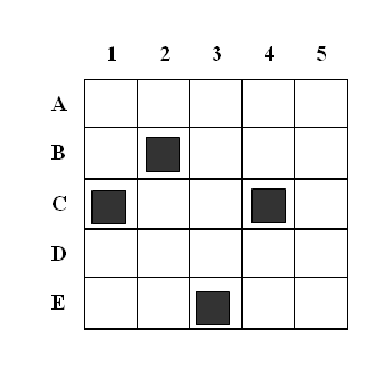
\includegraphics[scale=1]{motcroise.eps} 
\end{center}

\textbf{Horizontalement}\\

\noindent \textbf{A.}      $109 \times 100 + 4 \times 10 + 9$\\
\textbf{B.}        La partie entière de 5,02. /  Nombre entier compris entre 
519,9 et  520,2.\\
\textbf{C.}      Le nombre de centièmes dans 0,3. / Combien de nombres entiers y-t-il entre 1257,2 et 1265,9?\\
\textbf{D.}       Le nombre de millièmes dans $25 + \dfrac{7}{100} + \dfrac{4}{10} + \dfrac{1}{1000}$.\\
\textbf{E.}      Trois dizaines. /   6,6 dizaines.\\

\textbf{Verticalement}\\

\noindent \textbf{1.}      Le nombre de dixièmes dans $\dfrac{150}{100}$. / La partie entière de 23,264.\\
\textbf{2.}      Le chiffre des centièmes de 25,007. / Nombre entier compris 
entre 349,05 et 350 ,2.\\
\textbf{3.}      Le nombre de millièmes dans 9,504.\\
\textbf{4.}      420 dixièmes. /  0,76 centaines.\\
\textbf{5.}      $\dfrac{9081600}{100}$.\\


\vspace*{0.5cm}
$\rightarrow$ \textbf{Comparaison de deux nombres }\\

\vspace*{0.5cm}

\exo \\ Comparer avec les symboles <, > ou =.\\

\initqa \qa $\dfrac{63}{100}$ . . . . $\dfrac{21}{100}$\\

 \qa $\dfrac{927}{1000}$ . . . . $\dfrac{9}{10}$\\
 
  \qa $\dfrac{800}{100}$ . . . . $\dfrac{8}{10}$\\
  
   \qa $\dfrac{321}{1000}$ . . . . $\dfrac{33}{100}$\\
   
   \qa $\dfrac{51}{10}$ . . . . $\dfrac{\text{51 000}}{1000}$\\
   
   
   \exo \\ \\ Comparer avec les symboles <, > ou =.\\

\initqa \qa $8 + \dfrac{3}{10}$ . . . . $8 + \dfrac{7}{100}$\\
   
   \qa $1 + \dfrac{70}{100}$ . . . . $ \dfrac{17}{10}$\\
   
   \qa $12 + \dfrac{8}{10}$ . . . . $16 + \dfrac{2}{10}$\\
   
   \qa $51 + \dfrac{3}{10}$ . . . . $51 + \dfrac{29}{100}$\\
   
   \qa $17 -  \dfrac{8}{10}$ . . . . $17 + \dfrac{2}{100}$\\
   
   
   \exo \\ Comparer avec les symboles <, > ou =.\\

\initqa \qa $ 92 + \dfrac{15}{100}$ . . . . 92,015 \\

 \qa $\dfrac{7}{10}$ . . . . $\dfrac{700}{1000}$\\
 
  \qa $\dfrac{43}{100}$ . . . . $\dfrac{4}{10}$\\
  
   \qa 5,01 . . . . $5+\dfrac{1}{100}$\\
   
   \qa $\dfrac{7 859}{1000}$ . . . . $78 + \dfrac{59}{100}$\\
   
  
  \exo \\ Ranger dans l'ordre croissant les nombres suivants. \\

$ 5,4$ \hspace*{1cm} $ \dfrac{542}{100} + \dfrac{3}{1 000}$ \hspace*{1cm} $ \dfrac{53}{10} + \dfrac{9}{100}$ \hspace*{1cm}$ 538$ centièmes\hspace*{1cm} $ \dfrac{5470}{1 000}$\\
   
\hspace*{2cm} . . . .  < . . . . < . . . . < . . . . < . . . . \\

\exo \\ Donner un encadrement au centième près de chaque nombre.\\

\initqa 

\qa . . . . < 52,909 < . . . .\\

\qa . . . . < 2,633 < . . . .\\

\qa . . . . < 45,102 < . . . .\\


\qa . . . . < $\dfrac{2576}{1000}$ < . . . .\\



$\rightarrow$ \textbf{Repérage sur une demi-droite graduée}\\

\exo \\ Pour chaque axe gradué, indiquer les abscisses des points marqués.\\

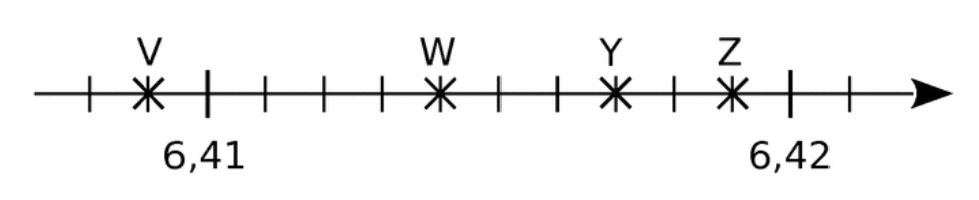
\includegraphics[scale=0.6]{graduee11.eps} \\

V( . . .) \hspace*{1cm} W( . . .)  \hspace*{1cm} Y( . . .) \hspace*{1cm} Z( . . .) \\


\exo \\ Pour chaque axe gradué, indiquer les abscisses des points marqués.\\

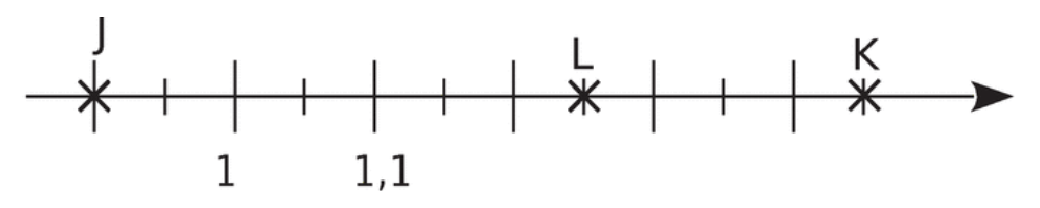
\includegraphics[scale=0.6]{graduee12.eps} \\

J( . . .) \hspace*{1cm} L( . . .)  \hspace*{1cm} K( . . .)  \\


\exo \\ Pour chaque axe gradué, indiquer les abscisses des points marqués.\\

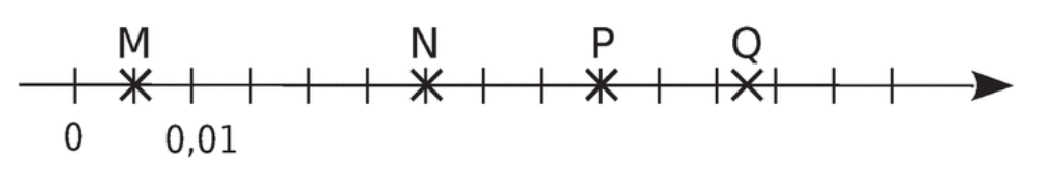
\includegraphics[scale=0.6]{graduee13.eps} \\

M( . . .) \hspace*{1cm} N( . . .)  \hspace*{1cm} P( . . .)  \hspace*{1cm} Q( . . .)\\

\vspace*{0.5cm}




\end{document}
